
\section{Measurement of Efficiency of Single Electron Trigger}

Single electron trigger, \texttt{HLT\_Ele27\_WPTight\_Gsf}, is used in $ee$, $e\mu$, $e\tau_h$, $e+jets$ channels.
In shape analysis, since the fitted template in $ee$ and $e+jets$ is based on the $p^T_e$ spectra, a pt dependent 
uncertainty of scale factors of \texttt{HLT\_Ele27\_WPTight\_Gsf} is needed to account for the trigger 
systematics properly of the templates of $p^T_e$ spectra. Here a customized measurement of scale factor and uncertainty
of \texttt{HLT\_Ele27\_WPTight\_Gsf} is performed using 2016 re-reco dataset with tag-prob approach. The uncertainty
of scale factor includes both statistical and systematical uncertainty, where systematical uncertainty are estimated by
"two shifts":

\begin{itemize}
  \item shift up the tagging electron by 10 GeV to effectively simulate a different trigger. This estimates the 
  systmatic effect that some L1 seed could have a threshold of 32 GeV.
  \item shift the probing electron pT up and down by 0.5 GeV. This etimates the effect of pT resolution.
\end{itemize}

The dataset used in the measurement is 2016 re-reco dataset SingleElectron/Run2016[B-H]-03Feb2017-*
with Golden Certificate as luminosity mask. The mc simulations used in the measurement are \texttt{DYJETSToLL\_M-10to50\_amcatnlo},
\texttt{DYJETSToLL\_M-50\_amcatnlo} and \texttt{TT\_powheg}, in which events reweighted to pile-up $\sigma_{mb} = 69.2\pm 2.3 mb$.

A standard tag-prob methord is used in the measurement of scale factor of \texttt{HLT\_Ele27\_WPTight\_Gsf}.
In electrons are selected with tight id and tight PF isolation with $p^T_e>20$ GeV and $|\eta_e|<2.5$. Corrections
to the electrons in the MC simulation includes energy scale-smear, reconstruction and isolation. Among selected electrons, tagged electrons
are defined as $p^T_e>30$ GeV and outside gap between barrel and endcap caolritmeters $1.444<|\eta_e|<1.56$, and 
match with \texttt{HLT\_Ele27\_WPTight\_Gsf} triggering objects. Events are selected by requring exactly 2
opposite electrons with at least 1 tagged electron and $60<m_{ee}<120$ GeV. This event selection yields a set of events 
significantly dominated by Drell-Yan process. The distribution of $m_{ee}$ is shown in fig~\ref{fig:appendix:ele27TriggerSF}.
The purity of Drell-Yan are very high in the selected events. Thus a signal-backgound fit is not necessary to get DY yields.



\begin{figure}
    \centering
    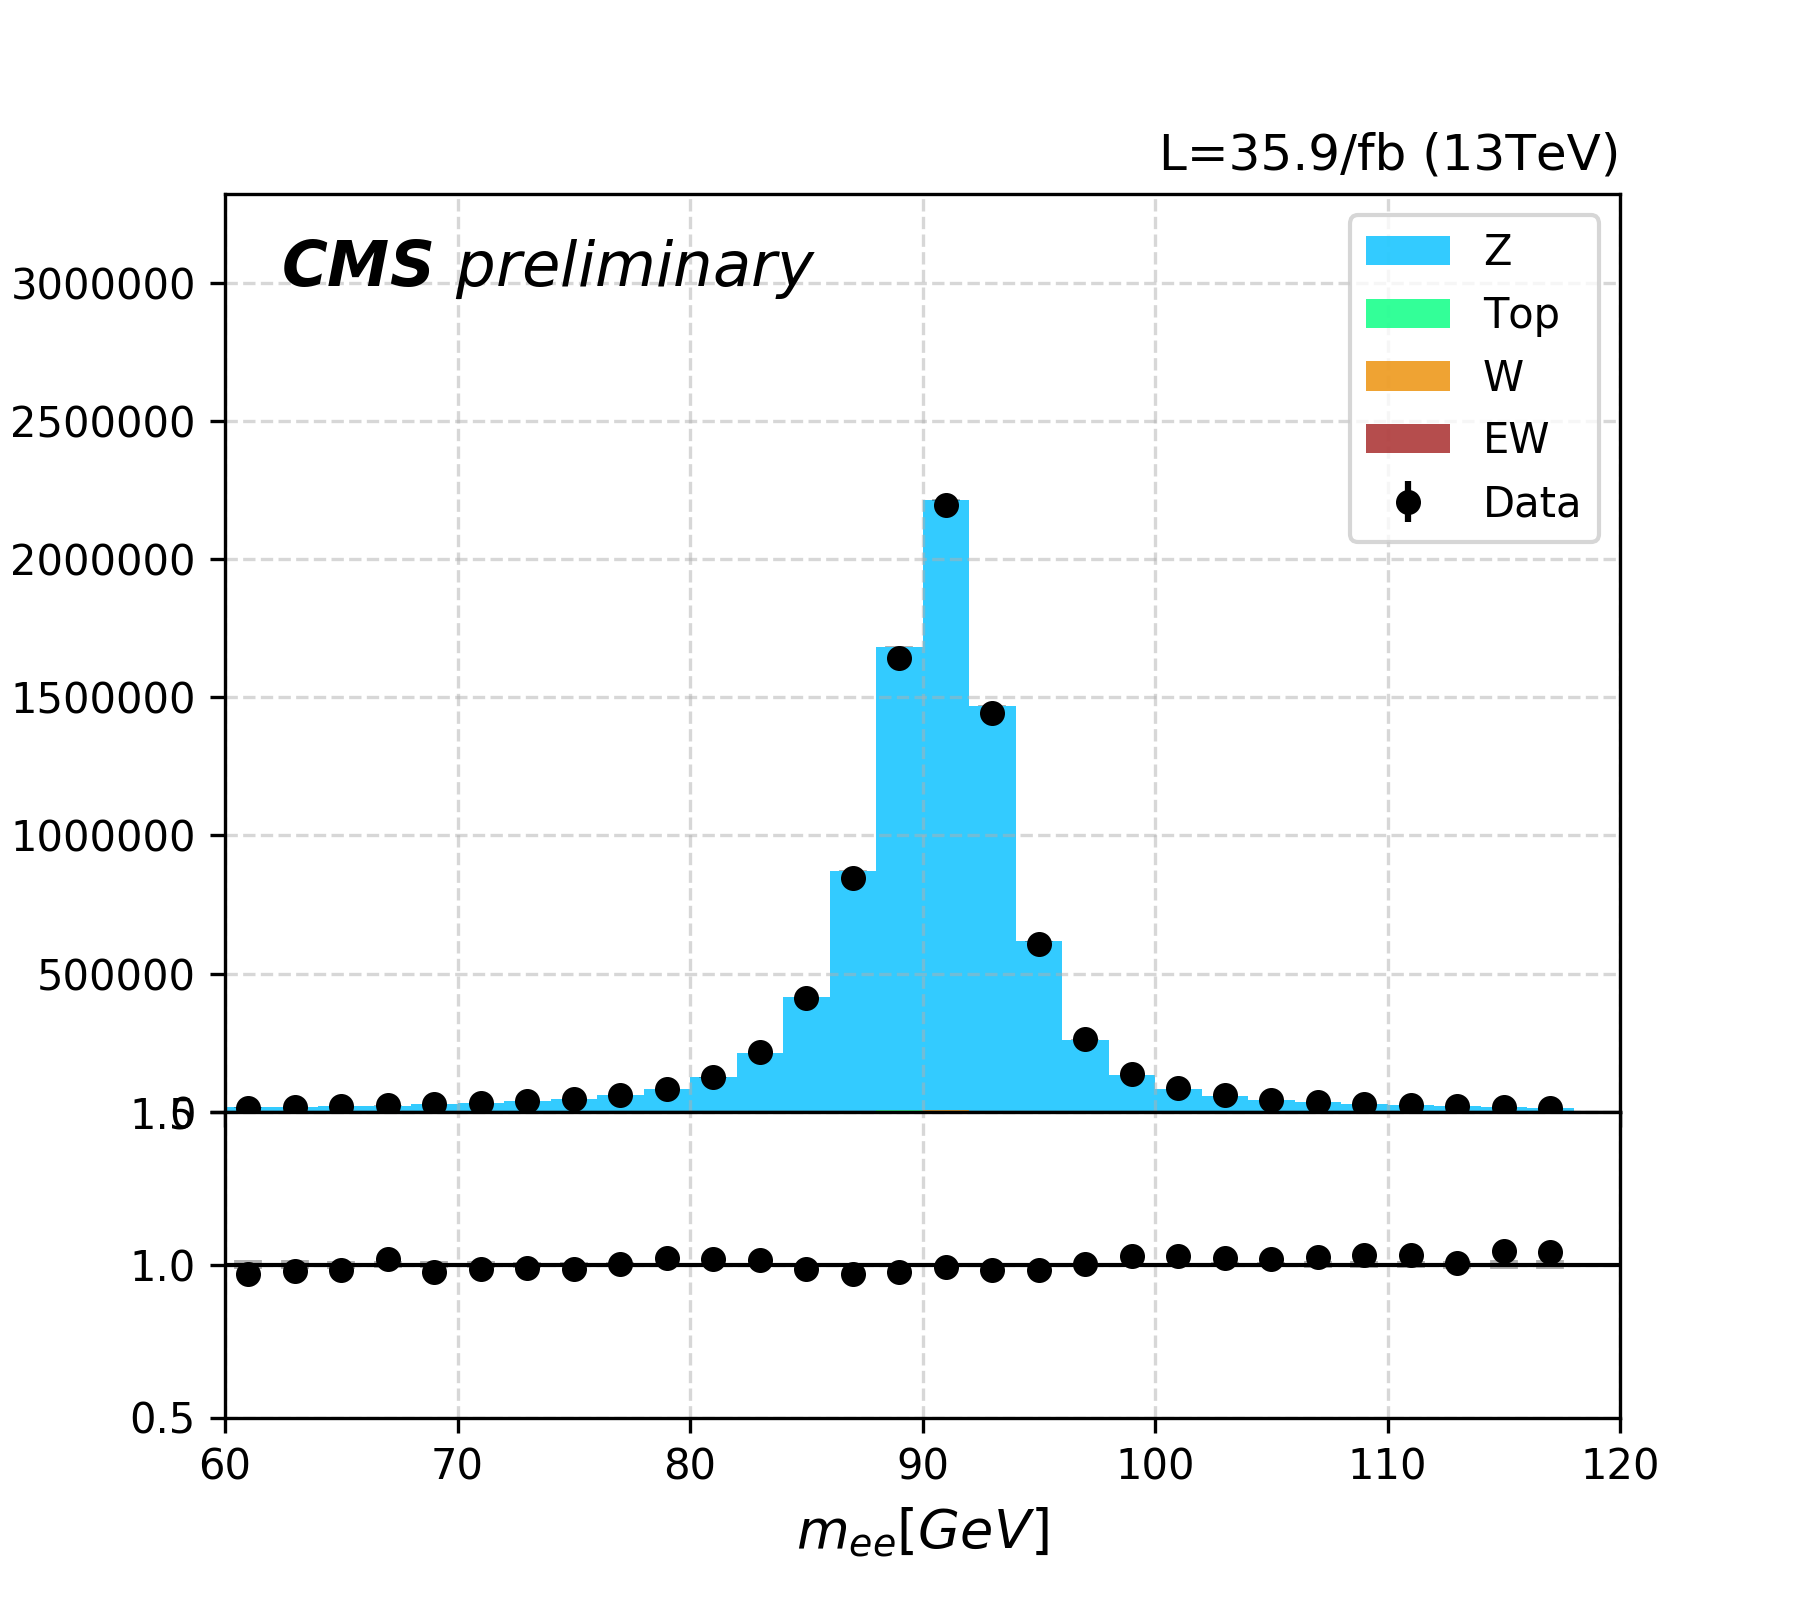
\includegraphics[width=0.6\textwidth]{chapters/Appendix/sectionEleTrigger/figures/dileptonMass_tag30.png}
    \caption{caption}
    \label{fig:appendix:ele27TriggerSF}
\end{figure}

In each event, if one electron is tagged, the other become a prob. Each event provides eigher 1 or 2 tag-prob pairs.
A prob is passing if it match with \texttt{HLT\_Ele27\_WPTight\_Gsf} triggering objects.
The trigger efficiencies are calculated by the ratio between number of passing tag-prob pairs and number of 
total tag-prob pairs in each $p^T_e-\eta_e$ bin. $\epsilon = \frac{ \text{\# passing tag-prob paris} } { \text{\# total tag-prob pairs}}$.
The scale factors are derived by taking the ratio between efficiencies of data over MC.
The scale factors are calcualted in 2D $p^T_e-\eta_e$ bins in each data taking periods and in B-F, GH combined periods.
The result of scale factors are shown in fig~\ref{fig:eTrSF_value}.

In 2016 B-F, the data efficiency in the endcap decreases because there is a decrease of signal over noise ratio associated 
to loss of	tracking hits caused by problems in the pre-amplifier of the APV chip. 
In the mid August 2016, this problem of Si-strip in endcap region is fixed by increase the drain speed of the pre-amplifier. Thus the 
trigger efficiencies are improved in 2016 GH. 


\begin{figure}
    \centering
    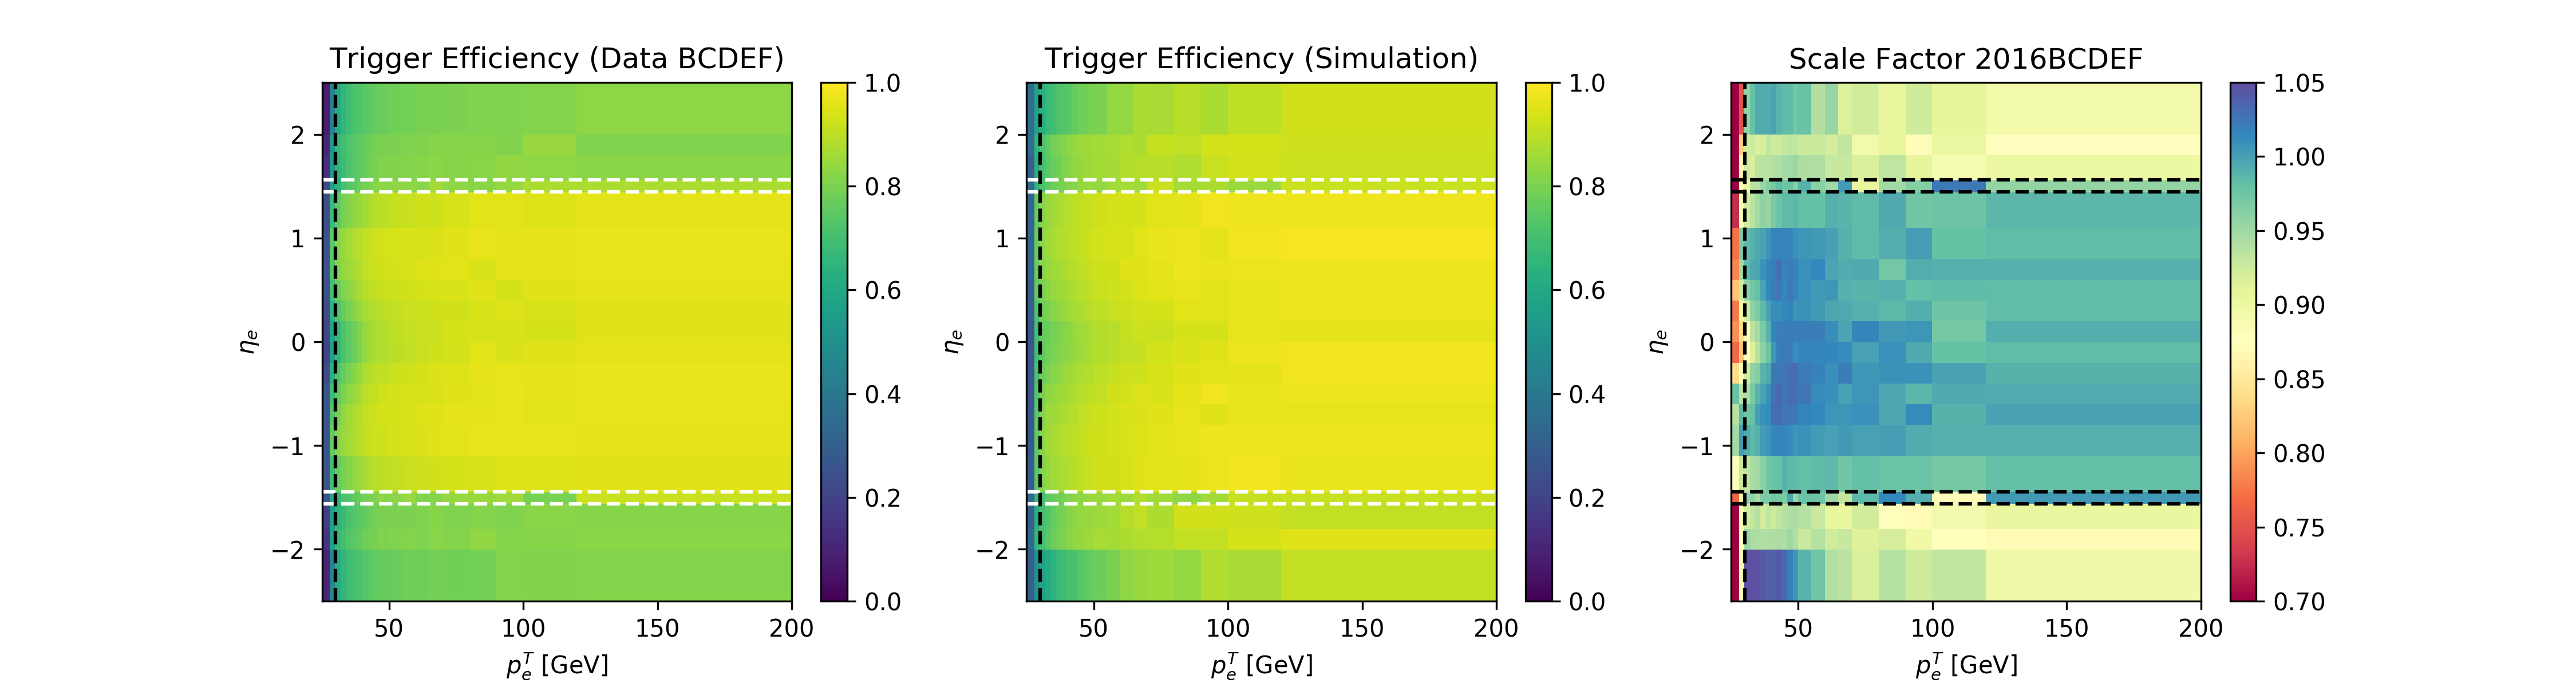
\includegraphics[width=0.99\textwidth]{chapters/Appendix/sectionEleTrigger/figures/eff2d_BCDEF.png}
    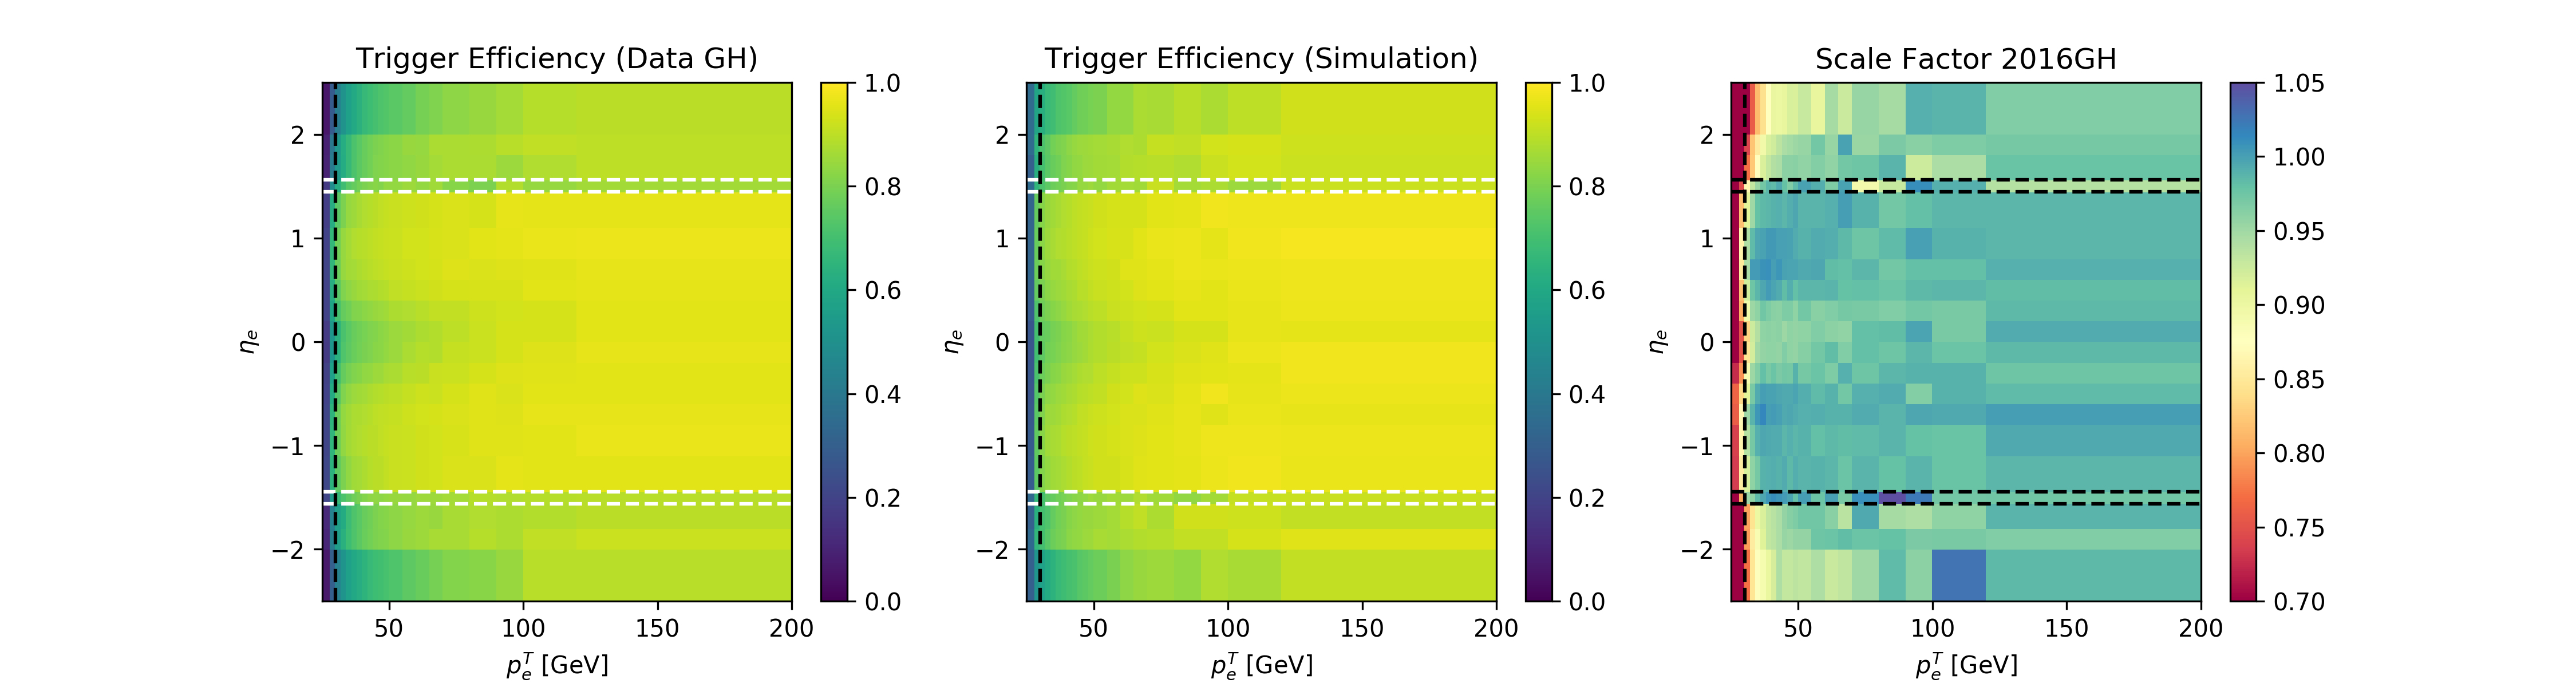
\includegraphics[width=0.99\textwidth]{chapters/Appendix/sectionEleTrigger/figures/eff2d_GH.png}
    \caption{Reweight $\tau_h$ and $j \to \tau_h$ efficiencies in the dedicated FSR, ISF, MEPS, UE ttbar samples}
    \label{fig:appendix:ele27SF}
\end{figure}



\begin{figure}
    \centering
    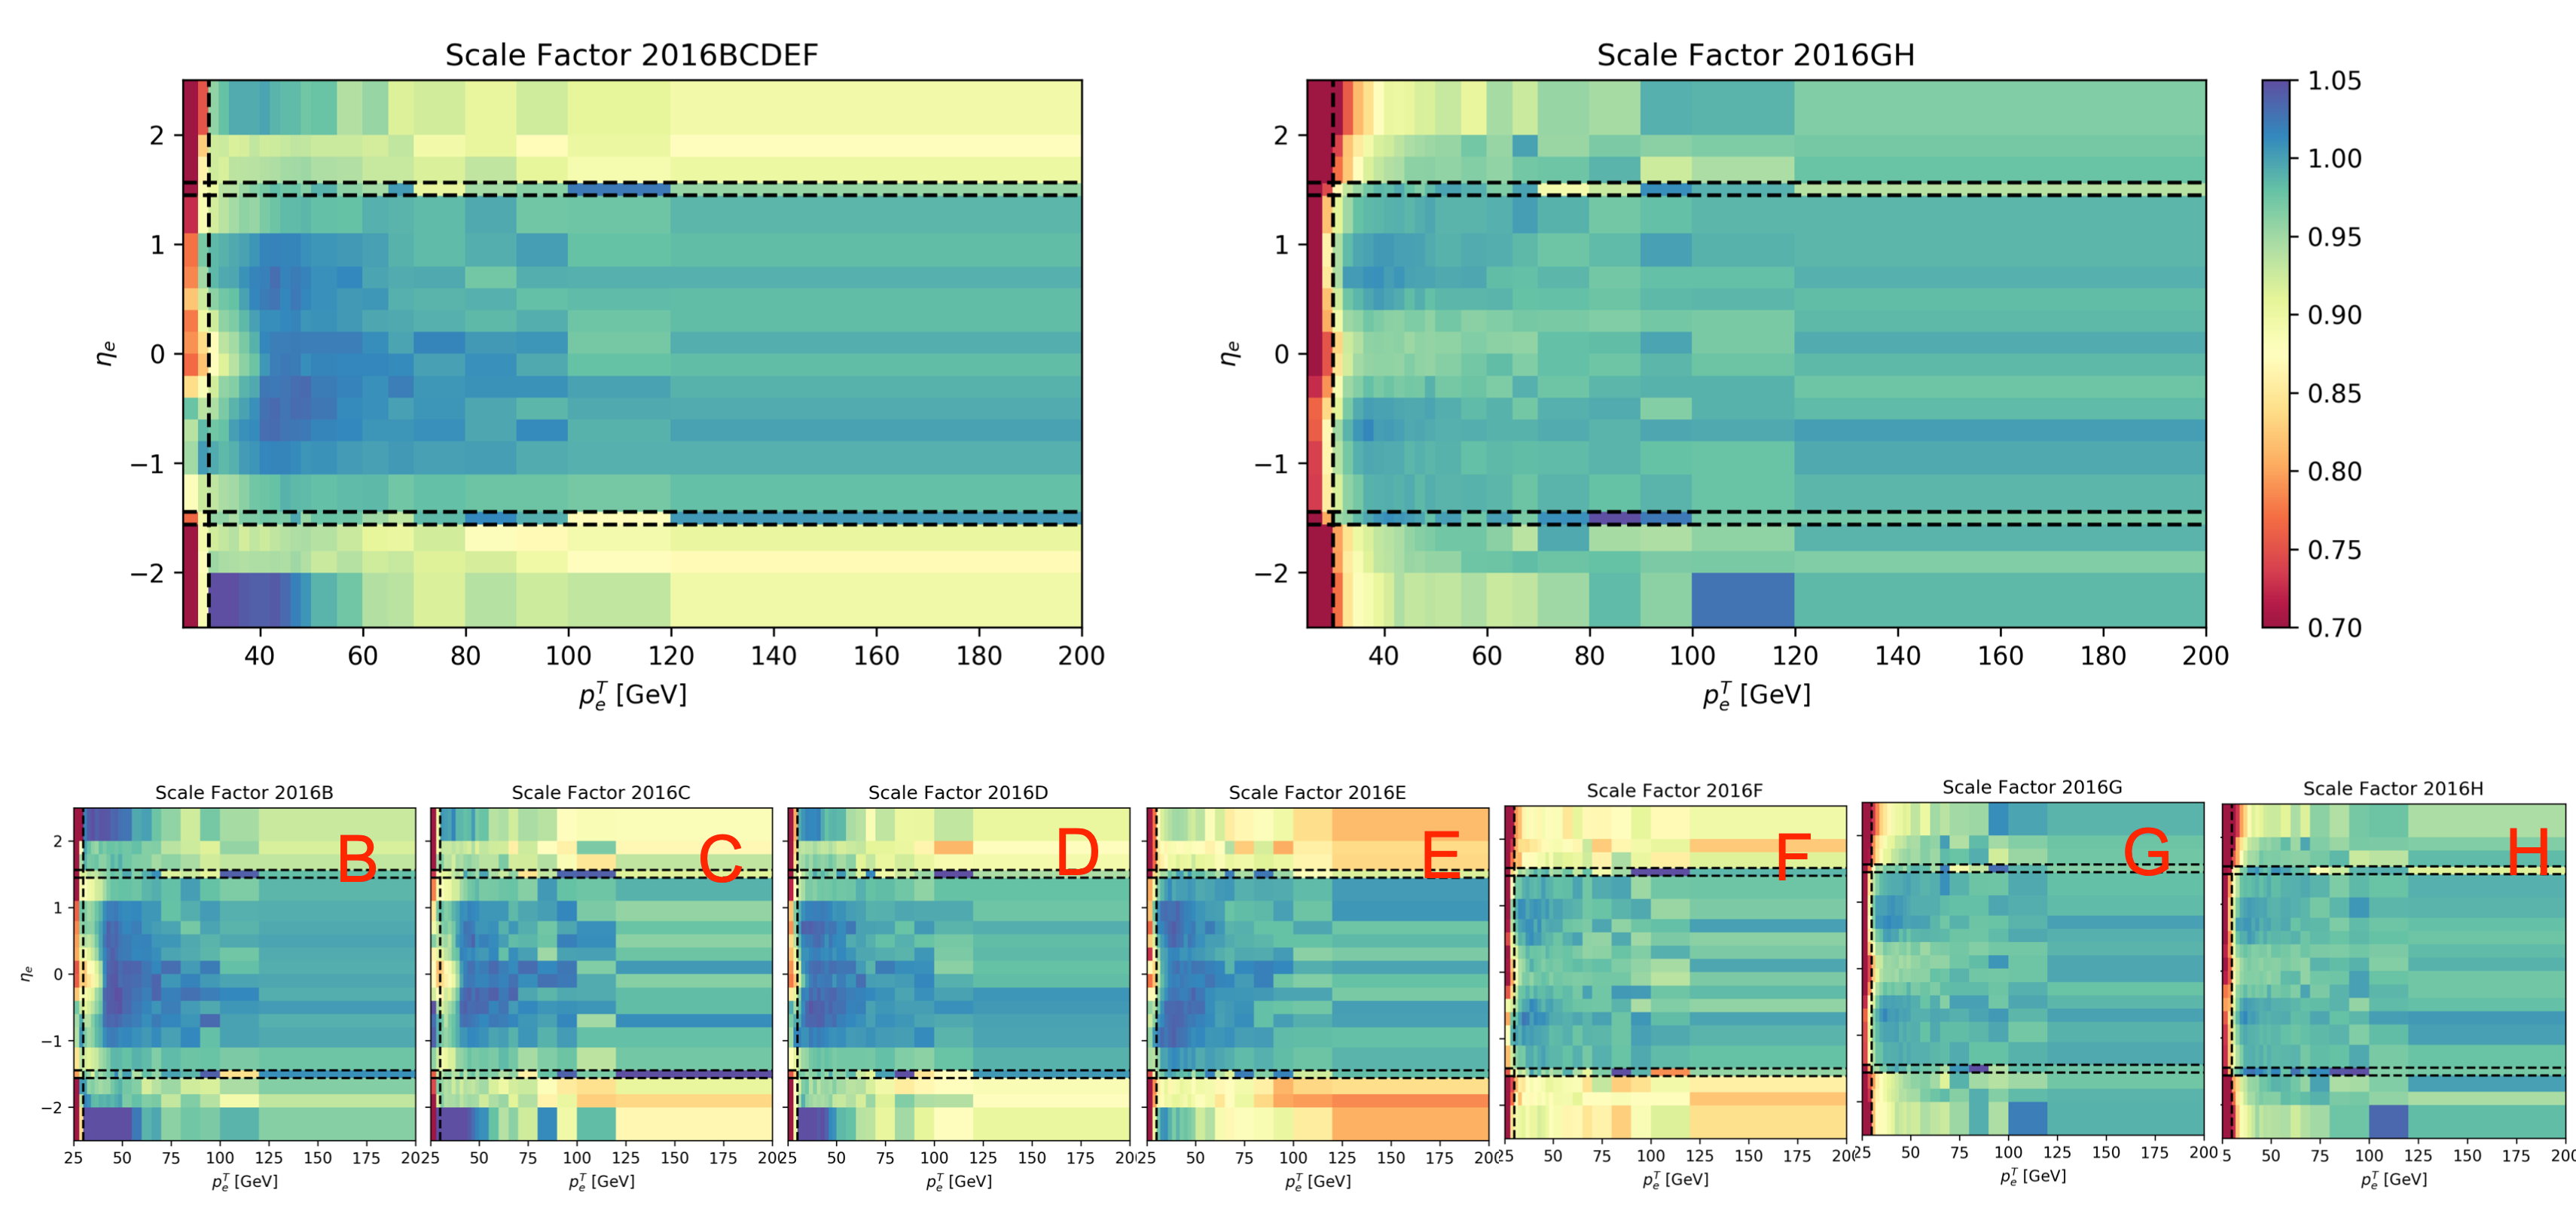
\includegraphics[width=0.99\textwidth]{chapters/Appendix/sectionEleTrigger/figures/eTrSF_value.png}
    \caption{Reweight $\tau_h$ and $j \to \tau_h$ efficiencies in the dedicated FSR, ISF, MEPS, UE ttbar samples}
    \label{fig:appendix:ele27SF}
\end{figure}




The total uncertainty of scale factors are quatic sum of statistical and systmatical uncertainties.
For 2016 B-F and GH, the total uncertainty and systmatical uncertainties from "two shifts" are shown
in fig~\ref{fig:eTrSF_err_BCDEF} ~\ref{fig:eTrSF_err_GH}.

\begin{figure}
    \centering
    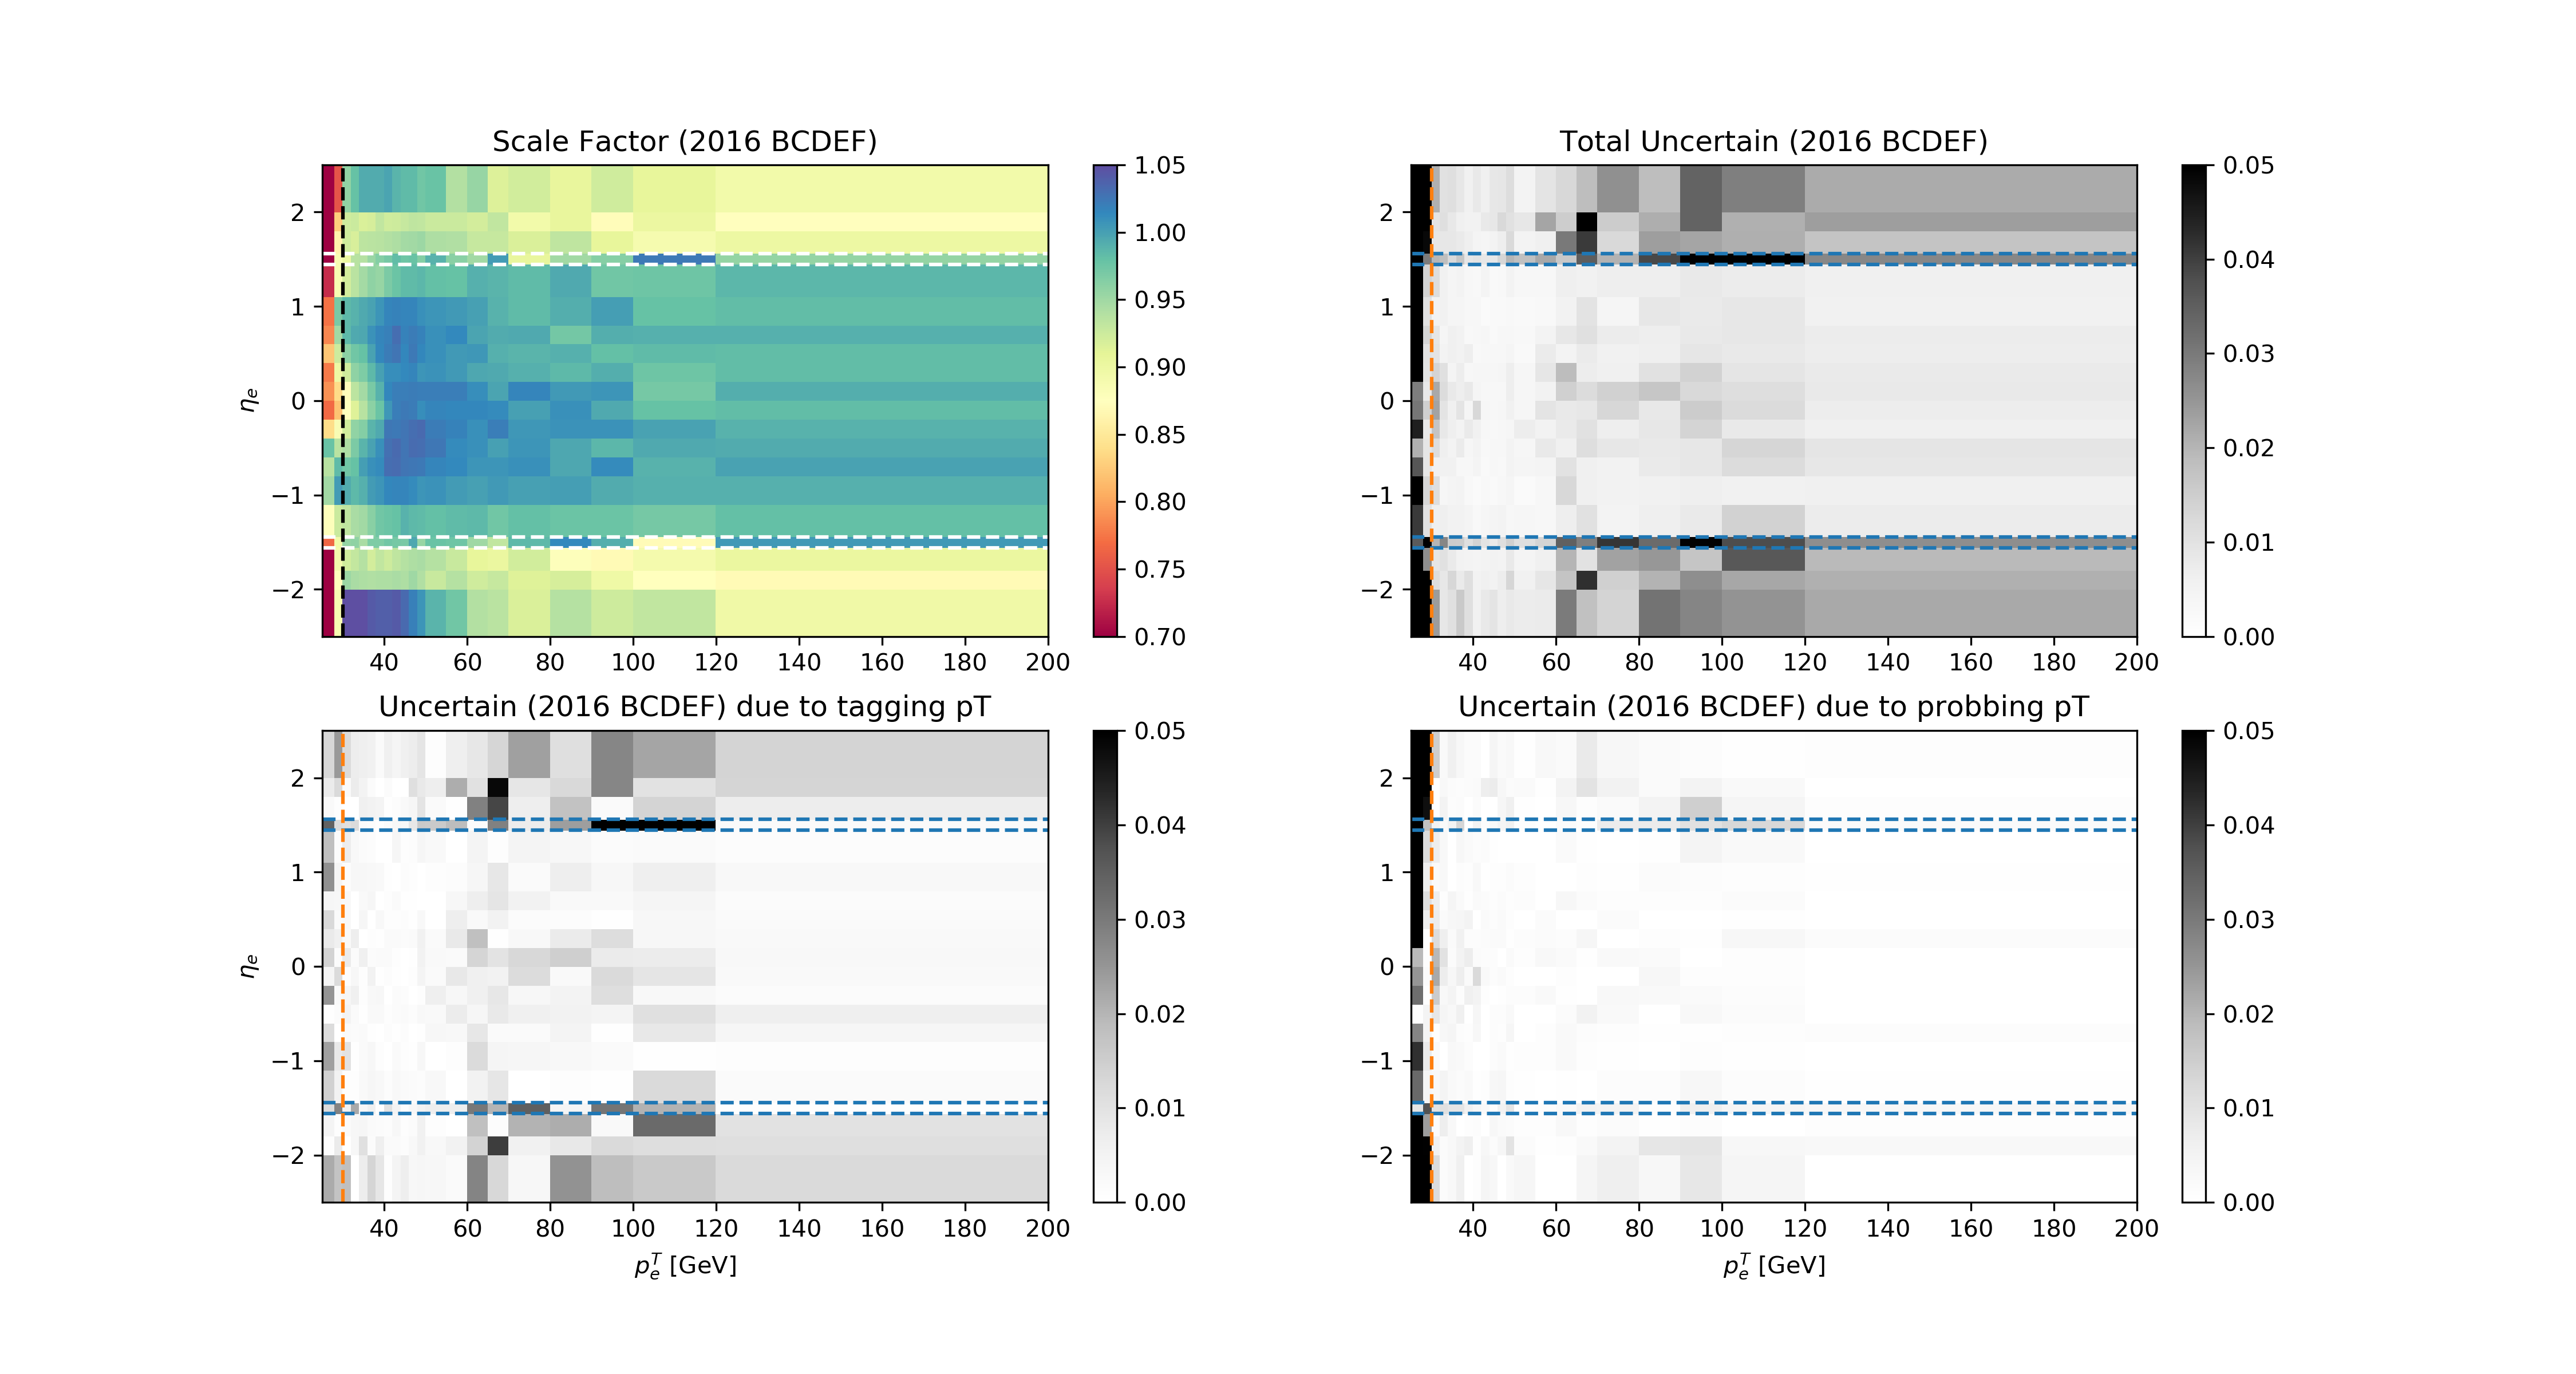
\includegraphics[width=0.99\textwidth]{chapters/Appendix/sectionEleTrigger/figures/result_BCDEF.png}
    
    \caption{caption}
    \label{fig:appendix:ele27SF}
\end{figure}

\begin{figure}
    \centering
    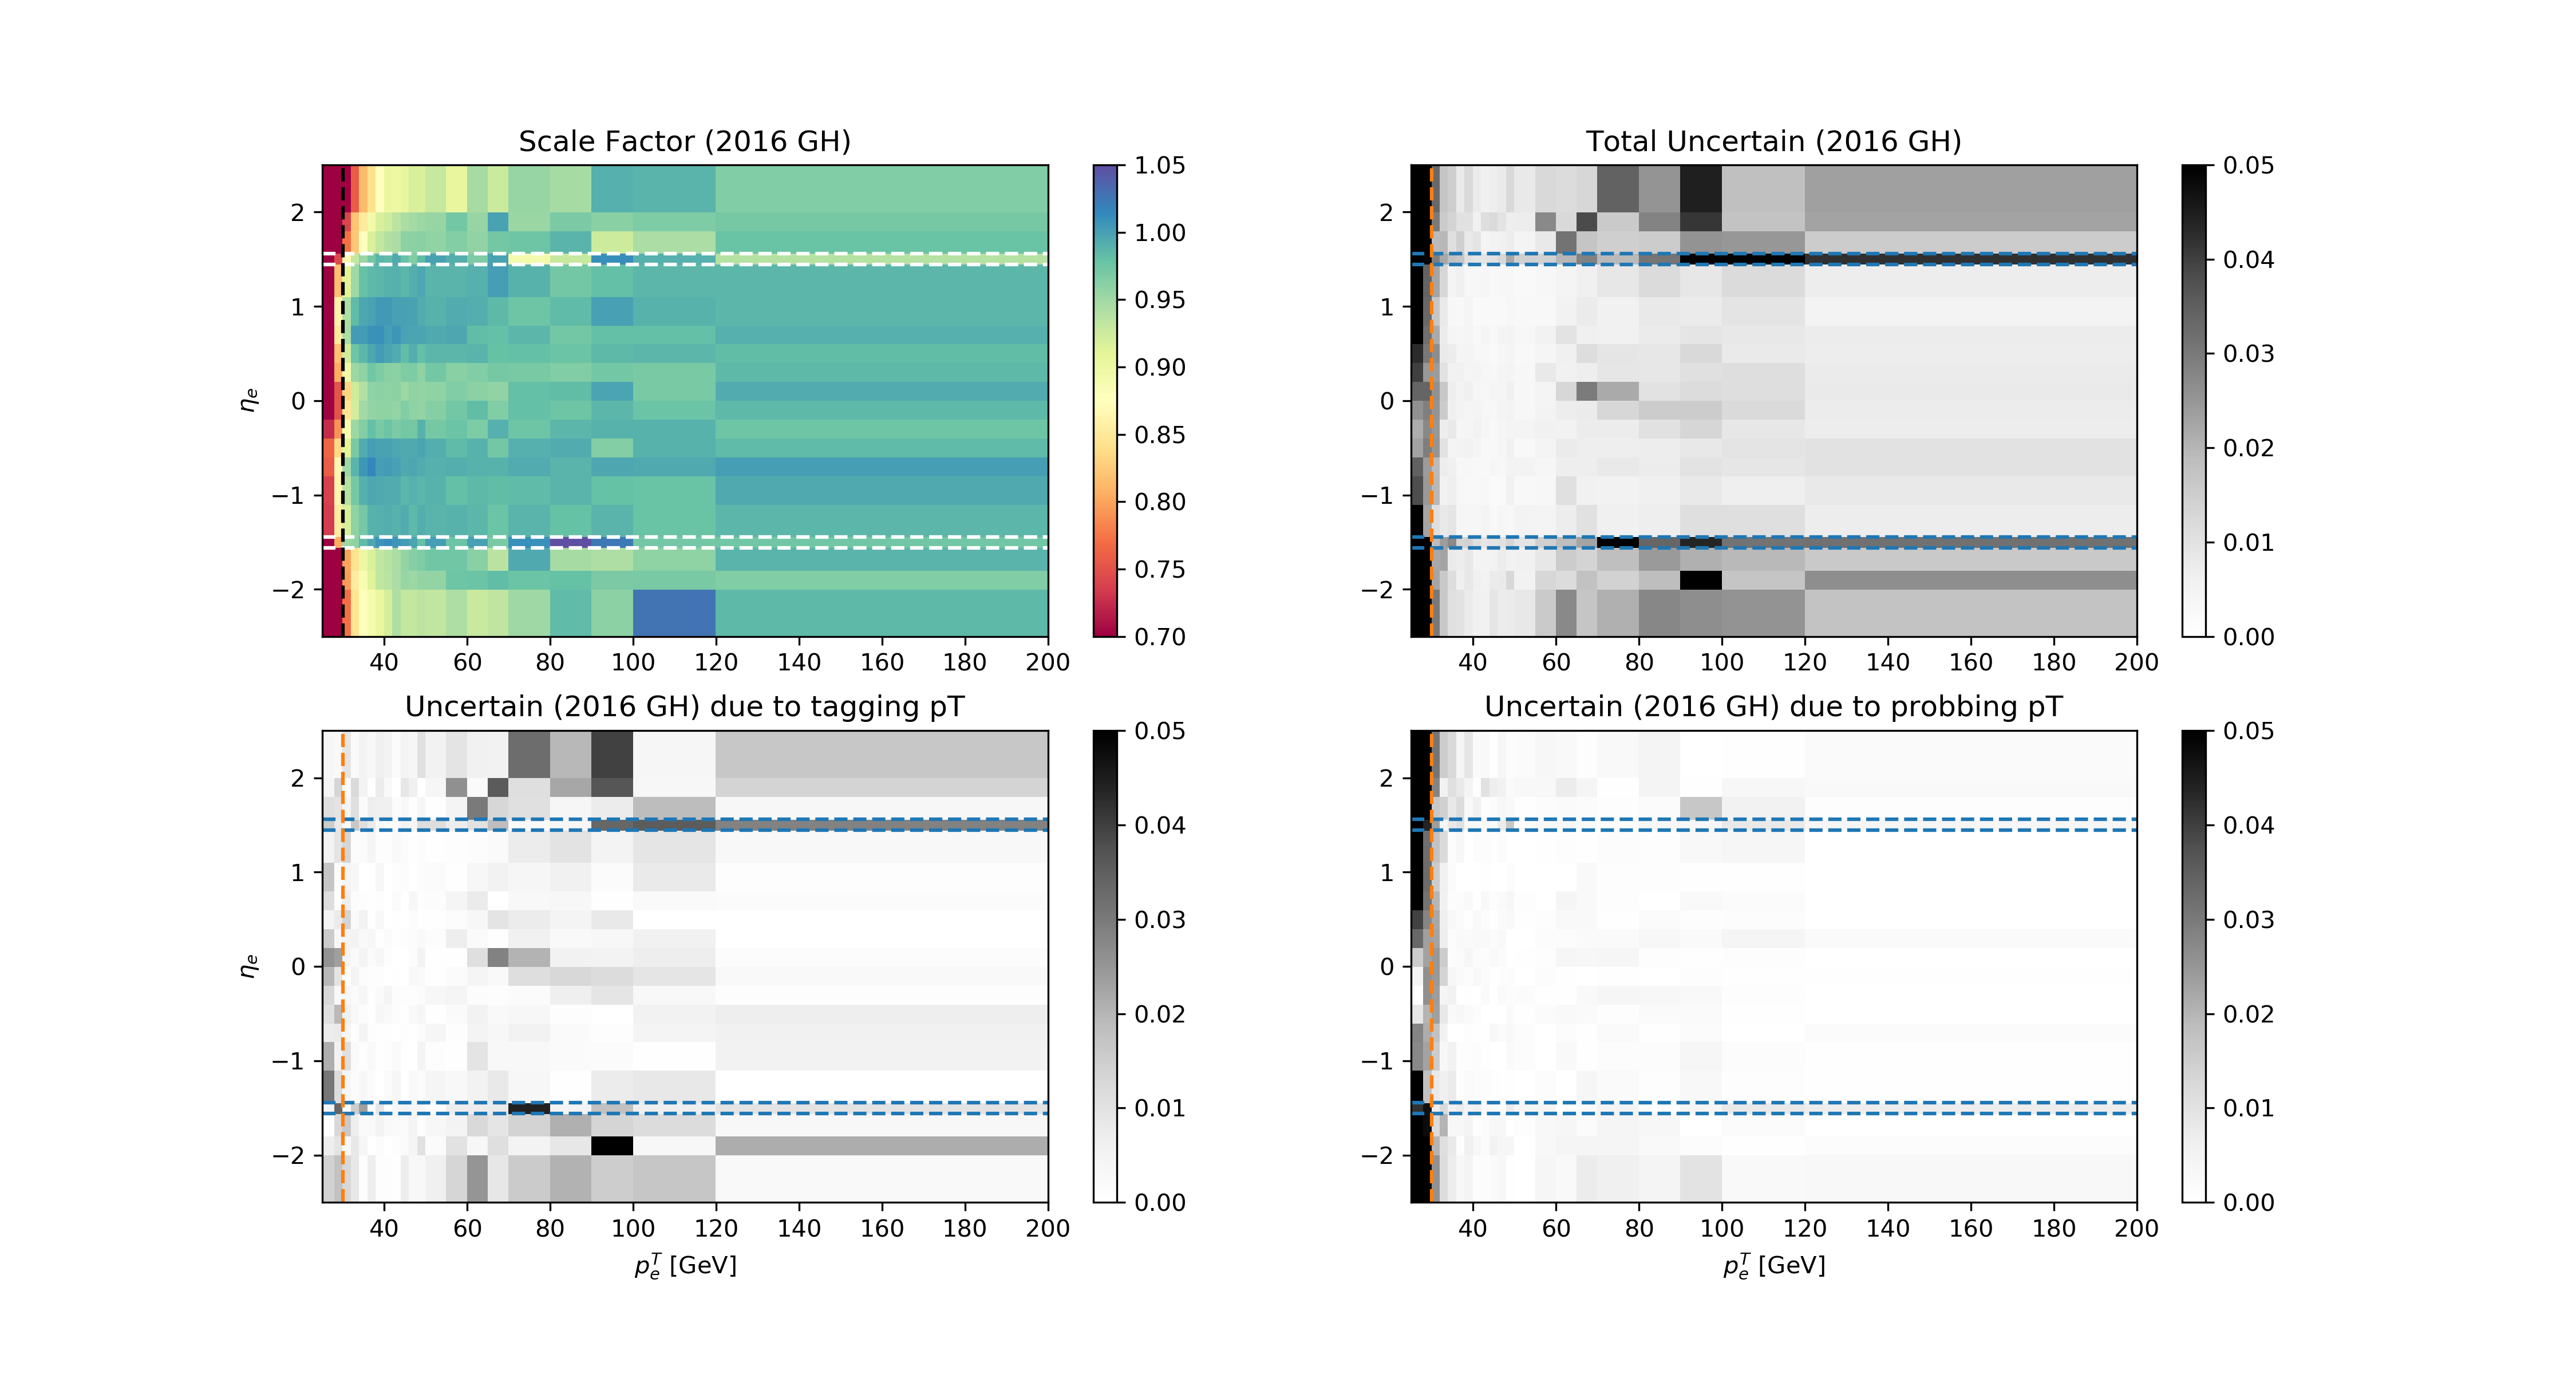
\includegraphics[width=0.99\textwidth]{chapters/Appendix/sectionEleTrigger/figures/result_GH.png}
    
    \caption{caption}
    \label{fig:appendix:ele27SF}
\end{figure}

\FloatBarrier
